\documentclass[letterpaper,12pt]{article}
\usepackage[margin=14mm,top=18mm,bottom=17mm,headheight=14pt]{geometry}
\pdfmapfile{+cm.map}\pdfmapfile{+cmextra.map}
\usepackage{tikz,fancyhdr,amsmath,amssymb}
\usetikzlibrary{arrows.meta,patterns}
\pagestyle{fancy}\fancyhf{}\renewcommand{\headrulewidth}{0pt}
\fancyhead[L]{\small Week 49 / Four-tower differences / Grades 2--3}
\fancyfoot[L]{\small Bellingham Math Circle / Week 49 / F49-23-v2}
\fancyfoot[R]{\small\thepage}
\setlength{\parindent}{0pt}\setlength{\parskip}{0pt}
\begin{document}
\noindent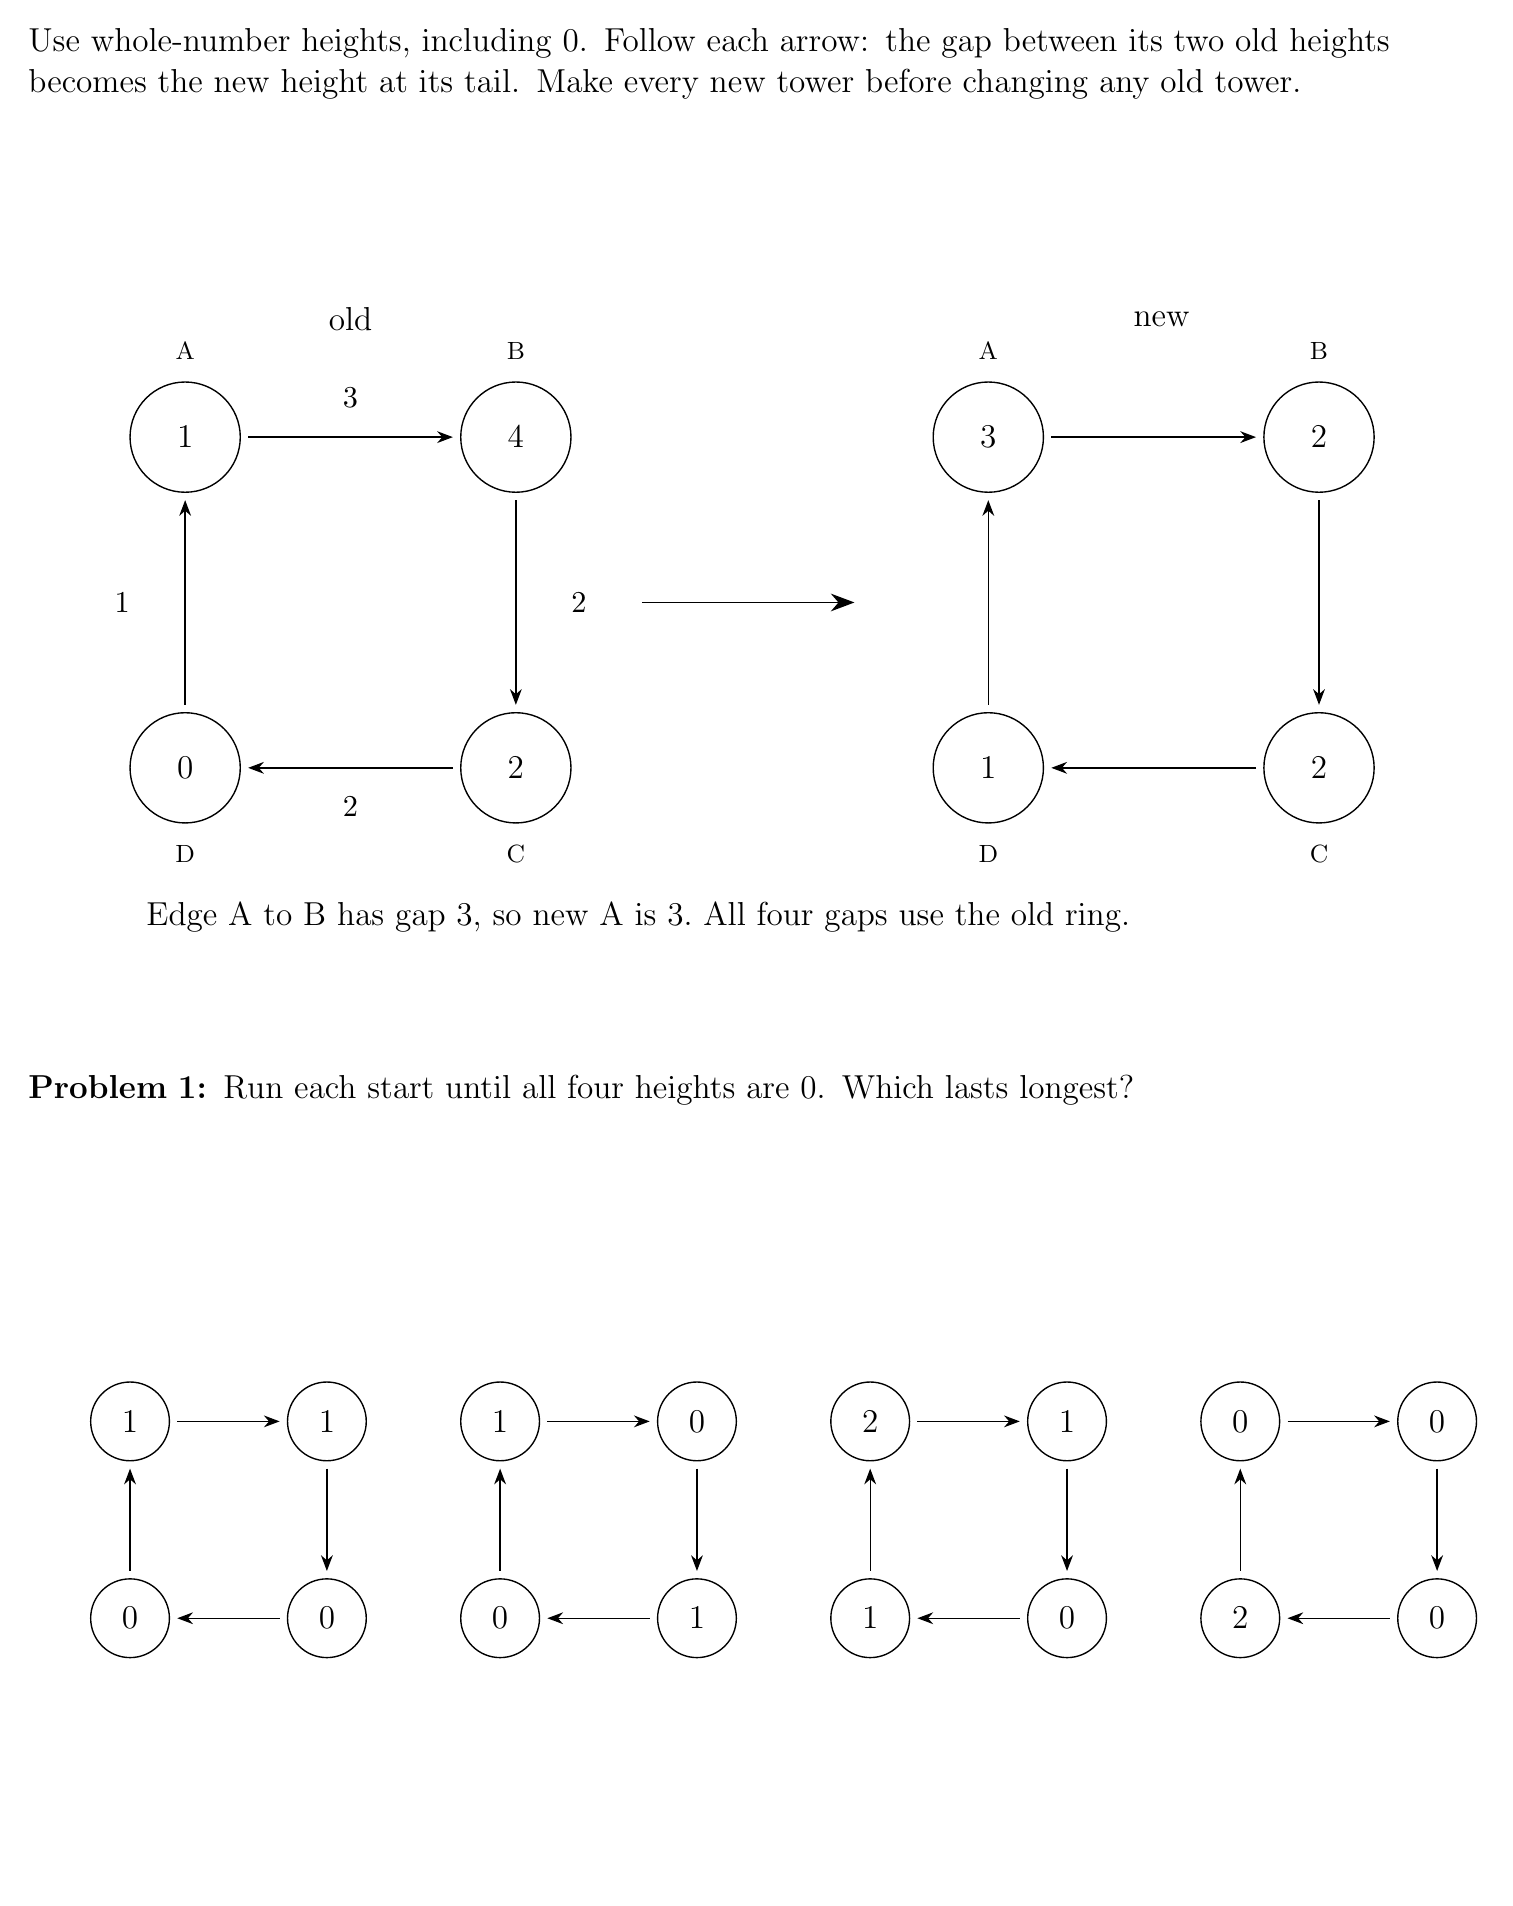
\begin{tikzpicture}[x=1mm,y=-1mm,line width=.5pt]
\path[use as bounding box] (0,0) rectangle (185,235);
\node[anchor=north west,inner sep=0pt,text width=180mm,font=\fontsize{12}{15}\selectfont] at (0,0) {Use whole-number heights, including 0. Follow each arrow: the gap between its two old heights becomes the new height at its tail. Make every new tower before changing any old tower.};
\node[anchor=center,inner sep=1pt,font=\fontsize{12}{14}\selectfont] at (41,37) {old};
\node[anchor=center,inner sep=1pt,font=\fontsize{12}{14}\selectfont] at (144,37) {new};
\draw[-{Stealth[length=2mm]}] (28.0,52.0) -- (54.0,52.0);
\node[anchor=center,inner sep=1pt,font=\fontsize{11}{13}\selectfont] at (41.0,47.0) {3};
\draw[-{Stealth[length=2mm]}] (62.0,60.0) -- (62.0,86.0);
\node[anchor=center,inner sep=1pt,font=\fontsize{11}{13}\selectfont] at (70.0,73.0) {2};
\draw[-{Stealth[length=2mm]}] (54.0,94.0) -- (28.0,94.0);
\node[anchor=center,inner sep=1pt,font=\fontsize{11}{13}\selectfont] at (41.0,99.0) {2};
\draw[-{Stealth[length=2mm]}] (20.0,86.0) -- (20.0,60.0);
\node[anchor=center,inner sep=1pt,font=\fontsize{11}{13}\selectfont] at (12.0,73.0) {1};
\draw[fill=white] (20,52) circle (7);
\node[anchor=center,inner sep=1pt,font=\fontsize{9}{11}\selectfont] at (20,41) {A};
\node[anchor=center,inner sep=1pt,font=\fontsize{13}{15}\selectfont] at (20,52) {1};
\draw[fill=white] (62,52) circle (7);
\node[anchor=center,inner sep=1pt,font=\fontsize{9}{11}\selectfont] at (62,41) {B};
\node[anchor=center,inner sep=1pt,font=\fontsize{13}{15}\selectfont] at (62,52) {4};
\draw[fill=white] (62,94) circle (7);
\node[anchor=center,inner sep=1pt,font=\fontsize{9}{11}\selectfont] at (62,105) {C};
\node[anchor=center,inner sep=1pt,font=\fontsize{13}{15}\selectfont] at (62,94) {2};
\draw[fill=white] (20,94) circle (7);
\node[anchor=center,inner sep=1pt,font=\fontsize{9}{11}\selectfont] at (20,105) {D};
\node[anchor=center,inner sep=1pt,font=\fontsize{13}{15}\selectfont] at (20,94) {0};
\draw[-{Stealth[length=3mm]}] (78,73) -- (105,73);
\draw[-{Stealth[length=2mm]}] (130.0,52.0) -- (156.0,52.0);
\draw[-{Stealth[length=2mm]}] (164.0,60.0) -- (164.0,86.0);
\draw[-{Stealth[length=2mm]}] (156.0,94.0) -- (130.0,94.0);
\draw[-{Stealth[length=2mm]}] (122.0,86.0) -- (122.0,60.0);
\draw[fill=white] (122,52) circle (7);
\node[anchor=center,inner sep=1pt,font=\fontsize{9}{11}\selectfont] at (122,41) {A};
\node[anchor=center,inner sep=1pt,font=\fontsize{13}{15}\selectfont] at (122,52) {3};
\draw[fill=white] (164,52) circle (7);
\node[anchor=center,inner sep=1pt,font=\fontsize{9}{11}\selectfont] at (164,41) {B};
\node[anchor=center,inner sep=1pt,font=\fontsize{13}{15}\selectfont] at (164,52) {2};
\draw[fill=white] (164,94) circle (7);
\node[anchor=center,inner sep=1pt,font=\fontsize{9}{11}\selectfont] at (164,105) {C};
\node[anchor=center,inner sep=1pt,font=\fontsize{13}{15}\selectfont] at (164,94) {2};
\draw[fill=white] (122,94) circle (7);
\node[anchor=center,inner sep=1pt,font=\fontsize{9}{11}\selectfont] at (122,105) {D};
\node[anchor=center,inner sep=1pt,font=\fontsize{13}{15}\selectfont] at (122,94) {1};
\node[anchor=north west,inner sep=0pt,text width=180mm,font=\fontsize{12}{15}\selectfont] at (15,111) {Edge A to B has gap 3, so new A is 3.\ All four gaps use the old ring.};
\node[anchor=north west,inner sep=0pt,text width=180mm,font=\fontsize{13}{16}\selectfont] at (0,133) {\textbf{Problem 1:} Run each start until all four heights are 0. Which lasts longest?};
\draw[-{Stealth[length=2mm]}] (19.0,177.0) -- (32.0,177.0);
\draw[-{Stealth[length=2mm]}] (38.0,183.0) -- (38.0,196.0);
\draw[-{Stealth[length=2mm]}] (32.0,202.0) -- (19.0,202.0);
\draw[-{Stealth[length=2mm]}] (13.0,196.0) -- (13.0,183.0);
\draw[fill=white] (13,177) circle (5);
\node[anchor=center,inner sep=1pt,font=\fontsize{13}{15}\selectfont] at (13,177) {1};
\draw[fill=white] (38,177) circle (5);
\node[anchor=center,inner sep=1pt,font=\fontsize{13}{15}\selectfont] at (38,177) {1};
\draw[fill=white] (38,202) circle (5);
\node[anchor=center,inner sep=1pt,font=\fontsize{13}{15}\selectfont] at (38,202) {0};
\draw[fill=white] (13,202) circle (5);
\node[anchor=center,inner sep=1pt,font=\fontsize{13}{15}\selectfont] at (13,202) {0};
\draw[-{Stealth[length=2mm]}] (66.0,177.0) -- (79.0,177.0);
\draw[-{Stealth[length=2mm]}] (85.0,183.0) -- (85.0,196.0);
\draw[-{Stealth[length=2mm]}] (79.0,202.0) -- (66.0,202.0);
\draw[-{Stealth[length=2mm]}] (60.0,196.0) -- (60.0,183.0);
\draw[fill=white] (60,177) circle (5);
\node[anchor=center,inner sep=1pt,font=\fontsize{13}{15}\selectfont] at (60,177) {1};
\draw[fill=white] (85,177) circle (5);
\node[anchor=center,inner sep=1pt,font=\fontsize{13}{15}\selectfont] at (85,177) {0};
\draw[fill=white] (85,202) circle (5);
\node[anchor=center,inner sep=1pt,font=\fontsize{13}{15}\selectfont] at (85,202) {1};
\draw[fill=white] (60,202) circle (5);
\node[anchor=center,inner sep=1pt,font=\fontsize{13}{15}\selectfont] at (60,202) {0};
\draw[-{Stealth[length=2mm]}] (113.0,177.0) -- (126.0,177.0);
\draw[-{Stealth[length=2mm]}] (132.0,183.0) -- (132.0,196.0);
\draw[-{Stealth[length=2mm]}] (126.0,202.0) -- (113.0,202.0);
\draw[-{Stealth[length=2mm]}] (107.0,196.0) -- (107.0,183.0);
\draw[fill=white] (107,177) circle (5);
\node[anchor=center,inner sep=1pt,font=\fontsize{13}{15}\selectfont] at (107,177) {2};
\draw[fill=white] (132,177) circle (5);
\node[anchor=center,inner sep=1pt,font=\fontsize{13}{15}\selectfont] at (132,177) {1};
\draw[fill=white] (132,202) circle (5);
\node[anchor=center,inner sep=1pt,font=\fontsize{13}{15}\selectfont] at (132,202) {0};
\draw[fill=white] (107,202) circle (5);
\node[anchor=center,inner sep=1pt,font=\fontsize{13}{15}\selectfont] at (107,202) {1};
\draw[-{Stealth[length=2mm]}] (160.0,177.0) -- (173.0,177.0);
\draw[-{Stealth[length=2mm]}] (179.0,183.0) -- (179.0,196.0);
\draw[-{Stealth[length=2mm]}] (173.0,202.0) -- (160.0,202.0);
\draw[-{Stealth[length=2mm]}] (154.0,196.0) -- (154.0,183.0);
\draw[fill=white] (154,177) circle (5);
\node[anchor=center,inner sep=1pt,font=\fontsize{13}{15}\selectfont] at (154,177) {0};
\draw[fill=white] (179,177) circle (5);
\node[anchor=center,inner sep=1pt,font=\fontsize{13}{15}\selectfont] at (179,177) {0};
\draw[fill=white] (179,202) circle (5);
\node[anchor=center,inner sep=1pt,font=\fontsize{13}{15}\selectfont] at (179,202) {0};
\draw[fill=white] (154,202) circle (5);
\node[anchor=center,inner sep=1pt,font=\fontsize{13}{15}\selectfont] at (154,202) {2};
\end{tikzpicture}
\newpage
\noindent\begin{tikzpicture}[x=1mm,y=-1mm,line width=.5pt]
\path[use as bounding box] (0,0) rectangle (185,235);
\node[anchor=north west,inner sep=0pt,text width=180mm,font=\fontsize{13}{16}\selectfont] at (0,0) {\textbf{Problem 2:} Choose starting heights from 0 to 5. Find a ring that lasts as many moves as you can. Count the move that first makes all four heights 0.};
\node[anchor=north west,inner sep=0pt,text width=180mm,font=\fontsize{11}{14}\selectfont] at (0,25) {An all-zero start takes 0 moves. Use these big mats for all four-station starts.};
\node[anchor=center,inner sep=1pt,font=\fontsize{12}{14}\selectfont] at (46,43) {old};
\node[anchor=center,inner sep=1pt,font=\fontsize{12}{14}\selectfont] at (139,43) {new};
\draw[-{Stealth[length=2mm]}] (41.0,71.0) -- (51.0,71.0);
\draw[-{Stealth[length=2mm]}] (72.0,92.0) -- (72.0,102.0);
\draw[-{Stealth[length=2mm]}] (51.0,123.0) -- (41.0,123.0);
\draw[-{Stealth[length=2mm]}] (20.0,102.0) -- (20.0,92.0);
\draw[fill=white,rounded corners=1mm] (0,51) rectangle ++(40,40);
\node[anchor=center,inner sep=1pt,font=\fontsize{9}{11}\selectfont] at (20,47) {A};
\draw[fill=white,rounded corners=1mm] (52,51) rectangle ++(40,40);
\node[anchor=center,inner sep=1pt,font=\fontsize{9}{11}\selectfont] at (72,47) {B};
\draw[fill=white,rounded corners=1mm] (52,103) rectangle ++(40,40);
\node[anchor=center,inner sep=1pt,font=\fontsize{9}{11}\selectfont] at (72,147) {C};
\draw[fill=white,rounded corners=1mm] (0,103) rectangle ++(40,40);
\node[anchor=center,inner sep=1pt,font=\fontsize{9}{11}\selectfont] at (20,147) {D};
\draw[-{Stealth[length=2mm]}] (134.0,71.0) -- (144.0,71.0);
\draw[-{Stealth[length=2mm]}] (165.0,92.0) -- (165.0,102.0);
\draw[-{Stealth[length=2mm]}] (144.0,123.0) -- (134.0,123.0);
\draw[-{Stealth[length=2mm]}] (113.0,102.0) -- (113.0,92.0);
\draw[fill=white,rounded corners=1mm] (93,51) rectangle ++(40,40);
\node[anchor=center,inner sep=1pt,font=\fontsize{9}{11}\selectfont] at (113,47) {A};
\draw[fill=white,rounded corners=1mm] (145,51) rectangle ++(40,40);
\node[anchor=center,inner sep=1pt,font=\fontsize{9}{11}\selectfont] at (165,47) {B};
\draw[fill=white,rounded corners=1mm] (145,103) rectangle ++(40,40);
\node[anchor=center,inner sep=1pt,font=\fontsize{9}{11}\selectfont] at (165,147) {C};
\draw[fill=white,rounded corners=1mm] (93,103) rectangle ++(40,40);
\node[anchor=center,inner sep=1pt,font=\fontsize{9}{11}\selectfont] at (113,147) {D};
\draw[] (20,176) rectangle ++(14,11);
\node[anchor=center,inner sep=1pt,font=\fontsize{12}{14}\selectfont] at (27,181.5) {};
\node[anchor=center,inner sep=1pt,font=\fontsize{9}{11}\selectfont] at (27,172) {A};
\draw[] (34,176) rectangle ++(14,11);
\node[anchor=center,inner sep=1pt,font=\fontsize{12}{14}\selectfont] at (41,181.5) {};
\node[anchor=center,inner sep=1pt,font=\fontsize{9}{11}\selectfont] at (41,172) {B};
\draw[] (48,176) rectangle ++(14,11);
\node[anchor=center,inner sep=1pt,font=\fontsize{12}{14}\selectfont] at (55,181.5) {};
\node[anchor=center,inner sep=1pt,font=\fontsize{9}{11}\selectfont] at (55,172) {C};
\draw[] (62,176) rectangle ++(14,11);
\node[anchor=center,inner sep=1pt,font=\fontsize{12}{14}\selectfont] at (69,181.5) {};
\node[anchor=center,inner sep=1pt,font=\fontsize{9}{11}\selectfont] at (69,172) {D};
\node[anchor=north west,inner sep=0pt,text width=85mm,font=\fontsize{12}{15}\selectfont] at (97,176) {Moves to zero: \rule{17mm}{.3pt}};
\draw[] (20,213) rectangle ++(14,11);
\node[anchor=center,inner sep=1pt,font=\fontsize{12}{14}\selectfont] at (27,218.5) {};
\node[anchor=center,inner sep=1pt,font=\fontsize{9}{11}\selectfont] at (27,209) {A};
\draw[] (34,213) rectangle ++(14,11);
\node[anchor=center,inner sep=1pt,font=\fontsize{12}{14}\selectfont] at (41,218.5) {};
\node[anchor=center,inner sep=1pt,font=\fontsize{9}{11}\selectfont] at (41,209) {B};
\draw[] (48,213) rectangle ++(14,11);
\node[anchor=center,inner sep=1pt,font=\fontsize{12}{14}\selectfont] at (55,218.5) {};
\node[anchor=center,inner sep=1pt,font=\fontsize{9}{11}\selectfont] at (55,209) {C};
\draw[] (62,213) rectangle ++(14,11);
\node[anchor=center,inner sep=1pt,font=\fontsize{12}{14}\selectfont] at (69,218.5) {};
\node[anchor=center,inner sep=1pt,font=\fontsize{9}{11}\selectfont] at (69,209) {D};
\node[anchor=north west,inner sep=0pt,text width=85mm,font=\fontsize{12}{15}\selectfont] at (97,213) {Moves to zero: \rule{17mm}{.3pt}};
\end{tikzpicture}
\newpage
\noindent\begin{tikzpicture}[x=1mm,y=-1mm,line width=.5pt]
\path[use as bounding box] (0,0) rectangle (185,235);
\node[anchor=north west,inner sep=0pt,text width=180mm,font=\fontsize{13}{16}\selectfont] at (0,0) {\textbf{Problem 3:} Could each ring be the result of one move? Find an old ring that makes it, or explain why no old ring can work.};
\draw[-{Stealth[length=2mm]}] (37.0,53.0) -- (59.0,53.0);
\draw[-{Stealth[length=2mm]}] (68.0,62.0) -- (68.0,84.0);
\draw[-{Stealth[length=2mm]}] (59.0,93.0) -- (37.0,93.0);
\draw[-{Stealth[length=2mm]}] (28.0,84.0) -- (28.0,62.0);
\draw[fill=white] (28,53) circle (8);
\node[anchor=center,inner sep=1pt,font=\fontsize{9}{11}\selectfont] at (28,41) {A};
\node[anchor=center,inner sep=1pt,font=\fontsize{13}{15}\selectfont] at (28,53) {2};
\draw[fill=white] (68,53) circle (8);
\node[anchor=center,inner sep=1pt,font=\fontsize{9}{11}\selectfont] at (68,41) {B};
\node[anchor=center,inner sep=1pt,font=\fontsize{13}{15}\selectfont] at (68,53) {0};
\draw[fill=white] (68,93) circle (8);
\node[anchor=center,inner sep=1pt,font=\fontsize{9}{11}\selectfont] at (68,105) {C};
\node[anchor=center,inner sep=1pt,font=\fontsize{13}{15}\selectfont] at (68,93) {2};
\draw[fill=white] (28,93) circle (8);
\node[anchor=center,inner sep=1pt,font=\fontsize{9}{11}\selectfont] at (28,105) {D};
\node[anchor=center,inner sep=1pt,font=\fontsize{13}{15}\selectfont] at (28,93) {0};
\draw[-{Stealth[length=2mm]}] (129.0,53.0) -- (151.0,53.0);
\draw[-{Stealth[length=2mm]}] (160.0,62.0) -- (160.0,84.0);
\draw[-{Stealth[length=2mm]}] (151.0,93.0) -- (129.0,93.0);
\draw[-{Stealth[length=2mm]}] (120.0,84.0) -- (120.0,62.0);
\draw[fill=white] (120,53) circle (8);
\node[anchor=center,inner sep=1pt,font=\fontsize{9}{11}\selectfont] at (120,41) {A};
\node[anchor=center,inner sep=1pt,font=\fontsize{13}{15}\selectfont] at (120,53) {1};
\draw[fill=white] (160,53) circle (8);
\node[anchor=center,inner sep=1pt,font=\fontsize{9}{11}\selectfont] at (160,41) {B};
\node[anchor=center,inner sep=1pt,font=\fontsize{13}{15}\selectfont] at (160,53) {1};
\draw[fill=white] (160,93) circle (8);
\node[anchor=center,inner sep=1pt,font=\fontsize{9}{11}\selectfont] at (160,105) {C};
\node[anchor=center,inner sep=1pt,font=\fontsize{13}{15}\selectfont] at (160,93) {1};
\draw[fill=white] (120,93) circle (8);
\node[anchor=center,inner sep=1pt,font=\fontsize{9}{11}\selectfont] at (120,105) {D};
\node[anchor=center,inner sep=1pt,font=\fontsize{13}{15}\selectfont] at (120,93) {0};
\draw[-{Stealth[length=2mm]}] (37.0,147.0) -- (59.0,147.0);
\draw[-{Stealth[length=2mm]}] (68.0,156.0) -- (68.0,178.0);
\draw[-{Stealth[length=2mm]}] (59.0,187.0) -- (37.0,187.0);
\draw[-{Stealth[length=2mm]}] (28.0,178.0) -- (28.0,156.0);
\draw[fill=white] (28,147) circle (8);
\node[anchor=center,inner sep=1pt,font=\fontsize{9}{11}\selectfont] at (28,135) {A};
\node[anchor=center,inner sep=1pt,font=\fontsize{13}{15}\selectfont] at (28,147) {1};
\draw[fill=white] (68,147) circle (8);
\node[anchor=center,inner sep=1pt,font=\fontsize{9}{11}\selectfont] at (68,135) {B};
\node[anchor=center,inner sep=1pt,font=\fontsize{13}{15}\selectfont] at (68,147) {1};
\draw[fill=white] (68,187) circle (8);
\node[anchor=center,inner sep=1pt,font=\fontsize{9}{11}\selectfont] at (68,199) {C};
\node[anchor=center,inner sep=1pt,font=\fontsize{13}{15}\selectfont] at (68,187) {1};
\draw[fill=white] (28,187) circle (8);
\node[anchor=center,inner sep=1pt,font=\fontsize{9}{11}\selectfont] at (28,199) {D};
\node[anchor=center,inner sep=1pt,font=\fontsize{13}{15}\selectfont] at (28,187) {1};
\draw[-{Stealth[length=2mm]}] (129.0,147.0) -- (151.0,147.0);
\draw[-{Stealth[length=2mm]}] (160.0,156.0) -- (160.0,178.0);
\draw[-{Stealth[length=2mm]}] (151.0,187.0) -- (129.0,187.0);
\draw[-{Stealth[length=2mm]}] (120.0,178.0) -- (120.0,156.0);
\draw[fill=white] (120,147) circle (8);
\node[anchor=center,inner sep=1pt,font=\fontsize{9}{11}\selectfont] at (120,135) {A};
\node[anchor=center,inner sep=1pt,font=\fontsize{13}{15}\selectfont] at (120,147) {0};
\draw[fill=white] (160,147) circle (8);
\node[anchor=center,inner sep=1pt,font=\fontsize{9}{11}\selectfont] at (160,135) {B};
\node[anchor=center,inner sep=1pt,font=\fontsize{13}{15}\selectfont] at (160,147) {0};
\draw[fill=white] (160,187) circle (8);
\node[anchor=center,inner sep=1pt,font=\fontsize{9}{11}\selectfont] at (160,199) {C};
\node[anchor=center,inner sep=1pt,font=\fontsize{13}{15}\selectfont] at (160,187) {0};
\draw[fill=white] (120,187) circle (8);
\node[anchor=center,inner sep=1pt,font=\fontsize{9}{11}\selectfont] at (120,199) {D};
\node[anchor=center,inner sep=1pt,font=\fontsize{13}{15}\selectfont] at (120,187) {2};
\end{tikzpicture}
\newpage
\noindent\begin{tikzpicture}[x=1mm,y=-1mm,line width=.5pt]
\path[use as bounding box] (0,0) rectangle (185,235);
\node[anchor=north west,inner sep=0pt,text width=180mm,font=\fontsize{13}{16}\selectfont] at (0,0) {\textbf{Problem 4:} Use the gap rule on both rings. Keep going until the whole ring repeats or becomes all zeros. Does the number of stations change what can happen?};
\draw[-{Stealth[length=2mm]}] (37.0,45.0) -- (51.0,45.0);
\draw[-{Stealth[length=2mm]}] (58.0,52.0) -- (58.0,66.0);
\draw[-{Stealth[length=2mm]}] (51.0,73.0) -- (37.0,73.0);
\draw[-{Stealth[length=2mm]}] (30.0,66.0) -- (30.0,52.0);
\draw[fill=white] (30,45) circle (6);
\node[anchor=center,inner sep=1pt,font=\fontsize{9}{11}\selectfont] at (30,35) {A};
\node[anchor=center,inner sep=1pt,font=\fontsize{13}{15}\selectfont] at (30,45) {1};
\draw[fill=white] (58,45) circle (6);
\node[anchor=center,inner sep=1pt,font=\fontsize{9}{11}\selectfont] at (58,35) {B};
\node[anchor=center,inner sep=1pt,font=\fontsize{13}{15}\selectfont] at (58,45) {0};
\draw[fill=white] (58,73) circle (6);
\node[anchor=center,inner sep=1pt,font=\fontsize{9}{11}\selectfont] at (58,83) {C};
\node[anchor=center,inner sep=1pt,font=\fontsize{13}{15}\selectfont] at (58,73) {0};
\draw[fill=white] (30,73) circle (6);
\node[anchor=center,inner sep=1pt,font=\fontsize{9}{11}\selectfont] at (30,83) {D};
\node[anchor=center,inner sep=1pt,font=\fontsize{13}{15}\selectfont] at (30,73) {0};
\draw[-{Stealth[length=2mm]}] (144.1304951684997,51.26099033699941) -- (151.8695048315003,66.73900966300059);
\draw[-{Stealth[length=2mm]}] (148.0,73.0) -- (134.0,73.0);
\draw[-{Stealth[length=2mm]}] (130.1304951684997,66.73900966300059) -- (137.8695048315003,51.26099033699941);
\draw[fill=white] (141.0,45) circle (6);
\node[anchor=center,inner sep=1pt,font=\fontsize{9}{11}\selectfont] at (141.0,35) {A};
\node[anchor=center,inner sep=1pt,font=\fontsize{13}{15}\selectfont] at (141.0,45) {1};
\draw[fill=white] (155,73) circle (6);
\node[anchor=center,inner sep=1pt,font=\fontsize{9}{11}\selectfont] at (155,83) {B};
\node[anchor=center,inner sep=1pt,font=\fontsize{13}{15}\selectfont] at (155,73) {0};
\draw[fill=white] (127,73) circle (6);
\node[anchor=center,inner sep=1pt,font=\fontsize{9}{11}\selectfont] at (127,83) {C};
\node[anchor=center,inner sep=1pt,font=\fontsize{13}{15}\selectfont] at (127,73) {0};
\node[anchor=center,inner sep=1pt,font=\fontsize{12}{14}\selectfont] at (46,91) {old};
\node[anchor=center,inner sep=1pt,font=\fontsize{12}{14}\selectfont] at (139,91) {new};
\draw[-{Stealth[length=2mm]}] (56.44721359549996,139.89442719099992) -- (61.55278640450004,150.10557280900008);
\draw[-{Stealth[length=2mm]}] (51.0,171.0) -- (41.0,171.0);
\draw[-{Stealth[length=2mm]}] (30.44721359549996,150.10557280900008) -- (35.55278640450004,139.89442719099992);
\draw[fill=white,rounded corners=1mm] (26.0,99) rectangle ++(40,40);
\node[anchor=center,inner sep=1pt,font=\fontsize{9}{11}\selectfont] at (46.0,95) {A};
\draw[fill=white,rounded corners=1mm] (52,151) rectangle ++(40,40);
\node[anchor=center,inner sep=1pt,font=\fontsize{9}{11}\selectfont] at (72,195) {B};
\draw[fill=white,rounded corners=1mm] (0,151) rectangle ++(40,40);
\node[anchor=center,inner sep=1pt,font=\fontsize{9}{11}\selectfont] at (20,195) {C};
\draw[-{Stealth[length=2mm]}] (149.44721359549996,139.89442719099992) -- (154.55278640450004,150.10557280900008);
\draw[-{Stealth[length=2mm]}] (144.0,171.0) -- (134.0,171.0);
\draw[-{Stealth[length=2mm]}] (123.44721359549996,150.10557280900008) -- (128.55278640450004,139.89442719099992);
\draw[fill=white,rounded corners=1mm] (119.0,99) rectangle ++(40,40);
\node[anchor=center,inner sep=1pt,font=\fontsize{9}{11}\selectfont] at (139.0,95) {A};
\draw[fill=white,rounded corners=1mm] (145,151) rectangle ++(40,40);
\node[anchor=center,inner sep=1pt,font=\fontsize{9}{11}\selectfont] at (165,195) {B};
\draw[fill=white,rounded corners=1mm] (93,151) rectangle ++(40,40);
\node[anchor=center,inner sep=1pt,font=\fontsize{9}{11}\selectfont] at (113,195) {C};
\end{tikzpicture}
\newpage
\noindent\begin{tikzpicture}[x=1mm,y=-1mm,line width=.5pt]
\path[use as bounding box] (0,0) rectangle (185,235);
\node[anchor=north west,inner sep=0pt,text width=180mm,font=\fontsize{13}{16}\selectfont] at (0,0) {\textbf{Problem 5:} Try different orders of 0, 1, 2, and 4. Which order lasts longest? Two rings count as different here only when their A, B, C, D heights differ.};
\draw[-{Stealth[length=2mm]}] (35.0,48.0) -- (57.0,48.0);
\draw[-{Stealth[length=2mm]}] (67.0,58.0) -- (67.0,80.0);
\draw[-{Stealth[length=2mm]}] (57.0,90.0) -- (35.0,90.0);
\draw[-{Stealth[length=2mm]}] (25.0,80.0) -- (25.0,58.0);
\draw[fill=white] (25,48) circle (9);
\node[anchor=center,inner sep=1pt,font=\fontsize{9}{11}\selectfont] at (25,35) {A};
\node[anchor=center,inner sep=1pt,font=\fontsize{13}{15}\selectfont] at (25,48) {0};
\draw[fill=white] (67,48) circle (9);
\node[anchor=center,inner sep=1pt,font=\fontsize{9}{11}\selectfont] at (67,35) {B};
\node[anchor=center,inner sep=1pt,font=\fontsize{13}{15}\selectfont] at (67,48) {1};
\draw[fill=white] (67,90) circle (9);
\node[anchor=center,inner sep=1pt,font=\fontsize{9}{11}\selectfont] at (67,103) {C};
\node[anchor=center,inner sep=1pt,font=\fontsize{13}{15}\selectfont] at (67,90) {2};
\draw[fill=white] (25,90) circle (9);
\node[anchor=center,inner sep=1pt,font=\fontsize{9}{11}\selectfont] at (25,103) {D};
\node[anchor=center,inner sep=1pt,font=\fontsize{13}{15}\selectfont] at (25,90) {4};
\draw[-{Stealth[length=2mm]}] (133.0,48.0) -- (155.0,48.0);
\draw[-{Stealth[length=2mm]}] (165.0,58.0) -- (165.0,80.0);
\draw[-{Stealth[length=2mm]}] (155.0,90.0) -- (133.0,90.0);
\draw[-{Stealth[length=2mm]}] (123.0,80.0) -- (123.0,58.0);
\draw[fill=white] (123,48) circle (9);
\node[anchor=center,inner sep=1pt,font=\fontsize{9}{11}\selectfont] at (123,35) {A};
\node[anchor=center,inner sep=1pt,font=\fontsize{13}{15}\selectfont] at (123,48) {0};
\draw[fill=white] (165,48) circle (9);
\node[anchor=center,inner sep=1pt,font=\fontsize{9}{11}\selectfont] at (165,35) {B};
\node[anchor=center,inner sep=1pt,font=\fontsize{13}{15}\selectfont] at (165,48) {1};
\draw[fill=white] (165,90) circle (9);
\node[anchor=center,inner sep=1pt,font=\fontsize{9}{11}\selectfont] at (165,103) {C};
\node[anchor=center,inner sep=1pt,font=\fontsize{13}{15}\selectfont] at (165,90) {4};
\draw[fill=white] (123,90) circle (9);
\node[anchor=center,inner sep=1pt,font=\fontsize{9}{11}\selectfont] at (123,103) {D};
\node[anchor=center,inner sep=1pt,font=\fontsize{13}{15}\selectfont] at (123,90) {2};
\node[anchor=north west,inner sep=0pt,text width=180mm,font=\fontsize{13}{16}\selectfont] at (0,127) {\textbf{Problem 6:} Can a new tower be taller than every old tower? Can the tallest height stay the same for a move? Give an explanation or an example for each claim.};
\draw[-{Stealth[length=2mm]}] (34.0,181.0) -- (58.0,181.0);
\draw[-{Stealth[length=2mm]}] (67.0,190.0) -- (67.0,214.0);
\draw[-{Stealth[length=2mm]}] (58.0,223.0) -- (34.0,223.0);
\draw[-{Stealth[length=2mm]}] (25.0,214.0) -- (25.0,190.0);
\draw[fill=white] (25,181) circle (8);
\node[anchor=center,inner sep=1pt,font=\fontsize{9}{11}\selectfont] at (25,169) {A};
\node[anchor=center,inner sep=1pt,font=\fontsize{13}{15}\selectfont] at (25,181) {0};
\draw[fill=white] (67,181) circle (8);
\node[anchor=center,inner sep=1pt,font=\fontsize{9}{11}\selectfont] at (67,169) {B};
\node[anchor=center,inner sep=1pt,font=\fontsize{13}{15}\selectfont] at (67,181) {1};
\draw[fill=white] (67,223) circle (8);
\node[anchor=center,inner sep=1pt,font=\fontsize{9}{11}\selectfont] at (67,235) {C};
\node[anchor=center,inner sep=1pt,font=\fontsize{13}{15}\selectfont] at (67,223) {2};
\draw[fill=white] (25,223) circle (8);
\node[anchor=center,inner sep=1pt,font=\fontsize{9}{11}\selectfont] at (25,235) {D};
\node[anchor=center,inner sep=1pt,font=\fontsize{13}{15}\selectfont] at (25,223) {4};
\draw[-{Stealth[length=2mm]}] (132.0,181.0) -- (156.0,181.0);
\draw[-{Stealth[length=2mm]}] (165.0,190.0) -- (165.0,214.0);
\draw[-{Stealth[length=2mm]}] (156.0,223.0) -- (132.0,223.0);
\draw[-{Stealth[length=2mm]}] (123.0,214.0) -- (123.0,190.0);
\draw[fill=white] (123,181) circle (8);
\node[anchor=center,inner sep=1pt,font=\fontsize{9}{11}\selectfont] at (123,169) {A};
\draw[fill=white] (165,181) circle (8);
\node[anchor=center,inner sep=1pt,font=\fontsize{9}{11}\selectfont] at (165,169) {B};
\draw[fill=white] (165,223) circle (8);
\node[anchor=center,inner sep=1pt,font=\fontsize{9}{11}\selectfont] at (165,235) {C};
\draw[fill=white] (123,223) circle (8);
\node[anchor=center,inner sep=1pt,font=\fontsize{9}{11}\selectfont] at (123,235) {D};
\end{tikzpicture}
\end{document}
